% =============================================================================
%  A proof of the Kauers--Koutschan conjecture for OEIS A216940
%  Alejandro Lizardi, 2026.
%
%  HOW TO COMPILE ON OVERLEAF
%  --------------------------
%  1. Create a new project and upload this file as the main .tex.
%  2. Upload the two images into an "assets/" subfolder:
%        assets/lockup.png  (Periapsis glyph+wordmark lockup, on the title page)
%        assets/mark.png    (Periapsis mark, in the page footer)
%     generated from periapsis-glyph-lockup.svg and periapsis-mark.svg.  If you
%     prefer the vector SVGs, enable \usepackage{svg} and use \includesvg.
%  3. Compiler: pdfLaTeX (default).  Uses only standard TeX Live packages
%     (amsmath, amsthm, tikz, algorithm/algpseudocode, fancyhdr, hyperref),
%     all present on Overleaf.
% =============================================================================
\documentclass[11pt]{article}

\usepackage[letterpaper,margin=1in,top=1in,bottom=1.1in]{geometry}
\usepackage[T1]{fontenc}
\usepackage{lmodern}
\usepackage{amsmath,amssymb,amsthm}
\usepackage{mathtools}
\usepackage{microtype}
\usepackage{booktabs}
\usepackage{array}
\usepackage{graphicx}
\usepackage{xcolor}
\usepackage{enumitem}
\usepackage{fancyhdr}
\usepackage{tikz}
\usetikzlibrary{positioning}
\usepackage{algorithm}
\usepackage{algpseudocode}
\usepackage[hidelinks]{hyperref}

% ---- To use the vector SVG mark instead of the PNG, comment the \includegraphics
% ---- line in the footer and use \includesvg (Overleaf has Inkscape enabled):
% \usepackage{svg}   % then \includesvg[height=34pt]{assets/periapsis-mark}

\definecolor{periapsisMuted}{HTML}{5A6068}

% ----- page footer: the Periapsis mark (only) in the bottom-right of every page
\pagestyle{fancy}
\fancyhf{}
\renewcommand{\headrulewidth}{0pt}
\renewcommand{\footrulewidth}{0pt}
\fancyfoot[R]{
\includegraphics[height=34pt]{assets/mark.png}}
\fancyfoot[C]{\color{periapsisMuted}\footnotesize\thepage}

% ----- theorem environments -------------------------------------------------
\theoremstyle{plain}
\newtheorem{theorem}{Theorem}
\newtheorem{proposition}[theorem]{Proposition}
\newtheorem{corollary}[theorem]{Corollary}
\newtheorem{lemma}[theorem]{Lemma}
\theoremstyle{definition}
\newtheorem{definition}[theorem]{Definition}
\newtheorem{conjecture}[theorem]{Conjecture}
\theoremstyle{remark}
\newtheorem{remark}[theorem]{Remark}

\newcommand{\OEIS}[1]{\texttt{#1}}
\newcommand{\Eseq}{\mathrm{E}}
\newcommand{\SW}{\mathrm{SW}}
\newcommand{\SE}{\mathrm{SE}}
\newcommand{\Om}{\Omega}
\newcommand{\des}{\operatorname{des}}

% =============================================================================
\begin{document}

% ----------------------------- TITLE BLOCK ----------------------------------
\thispagestyle{fancy}
\begin{center}
  {\LARGE\bfseries A proof of the Kauers--Koutschan conjecture\\[3pt]
   for the hexagonal Hardin array A216940\par}
  \vspace{14pt}
  {\large Alejandro Lizardi\par}
  \vspace{3pt}
  {\normalsize\href{mailto:alejlizardi05@gmail.com}{alejlizardi05@gmail.com}\par}
  \vspace{12pt}
  
\includegraphics[height=22pt]{assets/lockup.png}\par
  \vspace{10pt}
  {\small June 2026\par}
\end{center}

\vspace{6pt}
\begin{abstract}
\noindent The sequence \OEIS{A216940} of the On-Line Encyclopedia of Integer Sequences (OEIS)
counts the fillings of the side-$4$ hexagonal array with entries in $\{0,1,\dots,n\}$ that are
nondecreasing along the three directions east, south-west and south-east. Kauers and
Koutschan~(2023) proved that this sequence is a quasipolynomial in $n$ and conjectured an
explicit closed form for it (Conjecture~12 of their paper), which they were unable to derive
rigorously because the underlying partition-analysis computation did not terminate. We prove
their conjecture. The argument identifies $a(n)$ with the order polynomial $\Om_P(n+1)$ of an
explicit $37$-element poset $P$; a classical theorem of Stanley then gives, \emph{a priori},
that $a$ is a polynomial of degree exactly $37$. Computing $38$ values of $a$ directly from
$P$, independently of the conjectured formula, and matching them against Conjecture~12 forces
the two polynomials to coincide. The certificate is not a match against the published $37$-term
data, which is one value short of even determining a degree-$37$ polynomial; it rests on the a
priori degree bound together with one value beyond the published data. All computations are
reproducible.
\end{abstract}

\begin{center}\small
\textbf{MSC 2020:} 05A15, 06A07 (primary); 52B20 (secondary).\quad
\textbf{Keywords:} order polynomial; $P$-partition; Hardin array; D-finite sequence;
OEIS A216940; Ehrhart theory.
\end{center}

% ------------------------------- BODY ---------------------------------------
\section{Introduction}

In an automated study of sequences in the On-Line Encyclopedia of Integer Sequences (OEIS),
Kauers and Koutschan~\cite{KK23} singled out a family of sequences that are provably
$D$-finite but whose guessed recurrences or closed forms they could not establish rigorously.
One of these is \OEIS{A216940}, contributed to the OEIS by R.~H. Hardin~\cite{OEIS} in 2012
and described there as the ``number of side-$4$ hexagonal $0\dots n$ arrays with values
nondecreasing E, SW and SE.''

Concretely, write $H_4$ for the hexagonal patch of side $4$ drawn on the triangular grid: a
centrally symmetric hexagon whose seven rows have lengths $4,5,6,7,6,5,4$, for a total of $37$
cells. A \emph{filling} assigns to each cell a value in $\{0,1,\dots,n\}$; it is
\emph{admissible} if the values are weakly increasing along each of the three lattice
directions east ($\Eseq$), south-west ($\SW$) and south-east ($\SE$). Let $a(n)$ denote the
number of admissible fillings. The first values are
\[
  a(1)=260,\quad a(2)=27768,\quad a(3)=1664244,\quad a(4)=64697626,\ \dots
\]

Kauers and Koutschan proved (their Theorem~13) that $a$ is a quasipolynomial in $n$, hence
$D$-finite, by translating admissibility into a system of linear inequalities and invoking
partition analysis. They observed empirically that $a$ appears to be an honest polynomial, and
their LLL-based guesser produced an explicit candidate, which we restate.

\begin{conjecture}[Kauers--Koutschan {\cite[\S5.1]{KK23}}]\label{conj12}
With the raising-factorial notation $x^{\overline{k}}=x(x+1)\cdots(x+k-1)$,
\[
  a(n)\;=\;\frac{(n+1)^{\overline{13}}\,(n+6)^{\overline{3}}\,(n+7)\cdot q(n)}{D},
\]
where $q(n)=\sum_{i=0}^{20} c_i\,n^{i}$ is the explicit degree-$20$ integer polynomial with
$c_{20}=74384146$ and $c_0=15118483615575730790400000$ recorded in~\cite[\S5.1]{KK23}, and
$D=221424599279703105635713957232640000000$. The prefactor
$(n+1)^{\overline{13}}(n+6)^{\overline{3}}(n+7)$ has degree $13+3+1=17$, so the right-hand side
is a polynomial of total degree $37$.
\end{conjecture}

In the classification of~\cite[Table~1]{KK23}, \OEIS{A216940} carries the status \textbf{D}:
$D$-finiteness is proved, but the guessed closed form is not. The authors are explicit about
the obstruction~\cite[\S5.1]{KK23}:

\begin{quote}
``Again, we were not able to derive an expression by a rigorous computation based on partition
analysis, but we had no trouble to find a solution from our guessed recurrence. In fact, it
appears that the result is not only a quasipolynomial but a polynomial.''
\end{quote}

\paragraph{Result.} We prove Conjecture~\ref{conj12}, upgrading \OEIS{A216940} from status
\textbf{D} to \textbf{P}.

\begin{theorem}\label{main}
The number $a(n)$ of admissible fillings of the side-$4$ hexagonal array equals the right-hand
side of Conjecture~\ref{conj12}, identically as polynomials in $n$. In particular $a$ is a
polynomial of degree exactly $37$.
\end{theorem}

\subsection{A caveat about the data, and the shape of the proof}

It is tempting to argue that, since $a$ is ``known'' to be a polynomial, it suffices to match
Conjecture~\ref{conj12} against enough terms of the OEIS data. This is a trap. The published
b-file~\cite{OEIS} for \OEIS{A216940} lists exactly $37$ terms, $a(1),\dots,a(37)$. A
polynomial of degree $37$ has $38$ coefficients and is pinned by $38$ values;
\emph{thirty-seven values do not even determine it uniquely}, let alone prove a guessed form.
Moreover, the only route in the literature to an a priori degree bound is the
partition-analysis computation that Kauers--Koutschan report did not terminate. So a
term-match against the published data is not a proof, with zero margin to spare.

Our proof escapes this in two moves, set out in the sections that follow.
\begin{enumerate}[leftmargin=1.4em]
  \item \textbf{An a priori degree bound (Section~\ref{sec:degree}).} We exhibit $a$ as the
  order polynomial of an explicit finite poset. A classical theorem of Stanley then gives,
  with no reference to the conjecture, that $a$ is a polynomial of degree \emph{exactly} $37$.
  \item \textbf{One value beyond the data (Sections~\ref{sec:compute}--\ref{sec:proof}).} We
  compute $a(0),a(1),\dots,a(37)$---$38$ values---\emph{directly from the poset}, never using
  Conjecture~\ref{conj12}. The value $a(0)=1$ is genuinely new (it is not in the b-file).
  Matching all $38$ against Conjecture~\ref{conj12}, and invoking the degree bound, forces
  equality.
\end{enumerate}

\section{The hexagon as a poset}\label{sec:poset}

We use cube coordinates for the triangular grid: a cell is a triple $(x,y,z)\in\mathbb Z^3$
with $x+y+z=0$. The side-$s$ hexagon is
\[
  C_s \;=\;\{(x,y,z)\in\mathbb Z^3 : x+y+z=0,\ |x|,|y|,|z|\le s-1\},
  \qquad |C_s|=3s^2-3s+1.
\]
For $s=4$ this gives $|C_4|=3\cdot 16-12+1=37$ cells, arranged in rows (constant $z$) of
lengths $4,5,6,7,6,5,4$. The three monotonicity directions are the unit steps
\[
  \Eseq=(1,-1,0),\qquad \SW=(0,-1,1),\qquad \SE=(-1,0,1).
\]

\begin{definition}\label{def:poset}
Let $P_s=(C_s,\le)$ be the partial order generated by the relations $u\le u+\mathbf d$ for
$\mathbf d\in\{\Eseq,\SW,\SE\}$ whenever both $u$ and $u+\mathbf d$ lie in $C_s$; that is,
$\le$ is the reflexive--transitive closure of these steps. Write $P=P_4$.
\end{definition}

\begin{proposition}\label{prop:order}
$P_s$ is a partial order: the step relation is acyclic. An admissible filling of $H_s$ is
exactly an order-preserving map $P_s\to\{0,1,\dots,n\}$, i.e. a map $f$ with $f(u)\le f(v)$
whenever $u\le v$. Consequently
\[
  a(n)\;=\;\#\{\text{order-preserving } f:P\to\{0,\dots,n\}\}\;=\;\Om_P(n+1),
\]
where $\Om_P(m)$ is the order polynomial of $P$, the number of order-preserving maps from $P$
into the $m$-element chain $\{1,\dots,m\}$.
\end{proposition}

\begin{proof}
\emph{Acyclicity.} Along any step the coordinate $z$ is nondecreasing (it increases by $1$ on
$\SW$ and $\SE$ and is unchanged on $\Eseq$), and on an $\Eseq$-step within a fixed row the
coordinate $x$ strictly increases. Hence the map $(x,y,z)\mapsto(z,x)$ strictly increases
lexicographically along every step, so no nontrivial cycle of steps exists and the transitive
closure is a genuine partial order.

\emph{Identification.} Weak monotonicity along the three generating steps is, by transitivity,
exactly weak monotonicity along $\le$; so an admissible filling is the same as an
order-preserving map $P\to\{0,\dots,n\}$. Finally, such a map is the same as an
order-preserving map into the $(n+1)$-element chain $\{1,\dots,n+1\}$ after the shift
$f\mapsto f+1$, which is by definition counted by $\Om_P(n+1)$.
\end{proof}

\begin{remark}[covers versus generating steps]\label{rem:covers}
Not every generating step is a covering relation of $P$. Near the equator of the hexagon an
$\Eseq$-step coincides with the composite $\SW$-then-$\SE$, so that $\Eseq$-step is a
transitive, non-covering relation. For $s=4$ the $90$ generating steps comprise $60$ genuine
covers and $30$ transitive edges; the partial order---and hence $\Om_P$---depends only on the
transitive closure, so this distinction does not affect the count. We record it only so that
the Hasse diagram of $P$ is drawn correctly ($60$ edges, not $90$).
\end{remark}

\begin{figure}[ht]
\centering
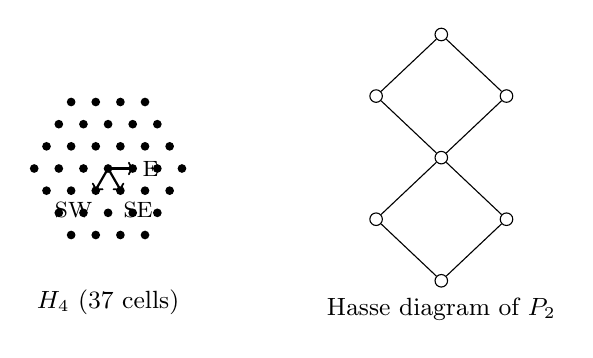
\begin{tikzpicture}[scale=0.92,every node/.style={font=\footnotesize}]
  % ---- left: the side-4 hexagon H_4 on the triangular grid ----
  \begin{scope}
    \def\r{0.34}
    \foreach \z [evaluate=\z as \w using {7-abs(\z)}] in {-3,-2,-1,0,1,2,3}{
      \foreach \k in {1,...,\w}{
        \pgfmathsetmacro\xoff{(\k-1) - (\w-1)/2}
        \fill[black] ({\xoff*\r},{-\z*\r*0.9}) circle (0.6mm);
      }
    }
    % direction arrows from the centre cell
    \draw[->,thick] (0,0)--({1.1*\r},0) node[right,xshift=-1pt]{$\Eseq$};
    \draw[->,thick] (0,0)--({-0.55*\r},{-0.95*\r}) node[below left,xshift=3pt]{$\SW$};
    \draw[->,thick] (0,0)--({0.55*\r},{-0.95*\r}) node[below right,xshift=-3pt]{$\SE$};
    \node[font=\small] at (0,-1.85) {$H_4$ (37 cells)};
  \end{scope}
  % ---- right: Hasse diagram of P_2 (the smallest nontrivial case) ----
  \begin{scope}[xshift=4.6cm,yshift=-1.55cm,every node/.style={circle,draw,inner sep=1.6pt,font=\scriptsize}]
    \node (min) at (0,0) {};
    \node (a1)  at (-0.9,0.85) {};
    \node (a2)  at ( 0.9,0.85) {};
    \node (mid) at (0,1.7) {};
    \node (b1)  at (-0.9,2.55) {};
    \node (b2)  at ( 0.9,2.55) {};
    \node (max) at (0,3.4) {};
    \draw (min)--(a1) (min)--(a2) (a1)--(mid) (a2)--(mid)
          (mid)--(b1) (mid)--(b2) (b1)--(max) (b2)--(max);
  \end{scope}
  \node[font=\small] at (4.6,-1.95) {Hasse diagram of $P_2$};
\end{tikzpicture}
\caption{Left: the side-$4$ hexagon $H_4$, $37$ cells in rows of lengths $4,5,6,7,6,5,4$, with
the three monotonicity directions $\Eseq,\SW,\SE$ marked. Right: the Hasse diagram of the
analogous side-$2$ poset $P_2$ (7 elements, 8 covers), shown as the smallest illustrative case;
$P_4$ has the same shape on $37$ elements with $60$ covers (Remark~\ref{rem:covers}).}
\label{fig:hexposet}
\end{figure}

\section{The a priori degree bound}\label{sec:degree}

The decisive structural input is classical and requires no computation.

\begin{theorem}[Stanley {\cite[\S3.15]{EC1}}]\label{thm:stanley-deg}
For any finite poset $P$ with $p$ elements, the order polynomial $\Om_P(m)$ is a polynomial in
$m$ of degree exactly $p$, with leading coefficient $e(P)/p!$, where $e(P)$ is the number of
linear extensions of $P$.
\end{theorem}

Combining Theorem~\ref{thm:stanley-deg} with Proposition~\ref{prop:order} yields the bound that
the data alone cannot supply.

\begin{corollary}\label{cor:deg37}
$a(n)=\Om_P(n+1)$ is a polynomial in $n$ of degree exactly $37$, with positive leading
coefficient $e(P)/37!$. In particular $a$ is a genuine polynomial (not merely a
quasipolynomial), confirming the empirical observation of~\cite{KK23}, and any two candidate
polynomials of degree $\le 37$ agreeing with $a$ at $38$ points are equal to $a$.
\end{corollary}

We stress that Corollary~\ref{cor:deg37} is independent of Conjecture~\ref{conj12}: it is a
statement about the order polynomial of $P$, proved before the conjectured coefficients are
ever consulted. This is the hinge on which the ``$37$ versus $38$'' difficulty turns. In
Section~\ref{sec:proof} we confirm the degree and the leading-coefficient identity numerically
as an internal check.

\section{Computing the order polynomial from the poset}\label{sec:compute}

It remains to compute $38$ values of $a$ directly from $P$. A na\"ive enumeration of
order-preserving maps $P\to\{0,\dots,n\}$ is hopeless for $n$ near $37$. Instead we compute $a$
through the descent statistic of the linear extensions of $P$, which is independent of $n$.

Fix a \emph{natural labelling} $\ell:P\to\{0,1,\dots,36\}$, i.e. an order-preserving bijection
onto $\{0,\dots,36\}$ (any linear extension serves; we use the one produced by Kahn's algorithm
with the smallest-index tie-break). A linear extension of $P$ is a permutation
$w=w_1w_2\cdots w_{37}$ of its elements that refines $\le$; its descent number is
$\des(w)=\#\{\,i:\ell(w_i)>\ell(w_{i+1})\,\}$. Let
$A_d=\#\{\text{linear extensions } w:\des(w)=d\}$.

\begin{theorem}[order polynomial via descents; Stanley {\cite[\S3.15.2]{EC1}}]\label{thm:descent}
With $p=|P|$ and $\{A_d\}$ as above,
\[
  \Om_P(m)\;=\;\sum_{d\ge 0} A_d\binom{m+p-1-d}{p},
  \qquad\text{hence}\qquad
  a(n)=\Om_P(n+1)=\sum_{d\ge 0} A_d\binom{n+p-d}{p}.
\]
\end{theorem}

The distribution $\{A_d\}$ is computed exactly, and without enumerating the (astronomically
many) individual linear extensions, by a transfer-matrix dynamic program over the \emph{order
ideals} (down-sets) of $P$ (Algorithm~\ref{alg:descent}). One builds a linear extension by
repeatedly appending a currently-minimal unplaced element; the only state needed to score the
next descent is the current ideal together with the label of the last placed element. The
number of reachable states is small---at most $10$ ideals at each rank level---so the program
is $n$-independent and runs in well under a second, returning the full distribution $\{A_d\}$
once and for all.

For $P=P_4$ the computation returns $e(P)=\sum_d A_d=4{,}623{,}718{,}515{,}360$ linear
extensions, with the descent distribution supported on $d=0,\dots,24$. The distribution is
\emph{palindromic}, $A_d=A_{24-d}$, with central value $A_{12}=1{,}048{,}272{,}112{,}322$ (the
full table is Appendix~\ref{app:cert}). Palindromy is the Ehrhart--reciprocity symmetry of the
order polytope $\mathcal O(P)$ and serves as an internal consistency check.

\section{Proof of Theorem~\ref{main}}\label{sec:proof}

\begin{proof}
By Proposition~\ref{prop:order}, $a(n)=\Om_P(n+1)$. By Corollary~\ref{cor:deg37}, $a$ is a
polynomial of degree exactly $37$; the right-hand side of Conjecture~\ref{conj12} is, by
inspection, also a polynomial of degree $37$. Two polynomials of degree $\le 37$ that agree at
$38$ distinct points are identical.

Using the descent distribution $\{A_d\}$ of Section~\ref{sec:compute} and the identity of
Theorem~\ref{thm:descent}, we evaluate
\[
  a(N)\;=\;\sum_{d=0}^{24} A_d\binom{N+37-d}{37},\qquad N=0,1,\dots,37,
\]
which gives $38$ values computed solely from the poset $P$---no coefficient of
Conjecture~\ref{conj12} enters this calculation. Independently, we evaluate the right-hand side
of Conjecture~\ref{conj12} at the same $38$ arguments. The two lists of $38$ integers coincide
exactly (Appendix~\ref{app:cert}, computed in exact rational arithmetic). The shared value at
$N=0$ is $a(0)=1$ (the unique constant filling), which lies beyond the published b-file and is
therefore a genuine $38$th datum, not a re-use of the OEIS data.

By the agreement at $38$ points and the degree bound, $a(n)$ and the right-hand side of
Conjecture~\ref{conj12} are the same polynomial.
\end{proof}

\begin{remark}\label{rem:leadcoef}
The leading coefficient supplied by Corollary~\ref{cor:deg37},
$e(P)/37!=4{,}623{,}718{,}515{,}360/37!$, agrees with the leading coefficient of
Conjecture~\ref{conj12} computed symbolically. This is an independent cross-check of both the
degree bound and the descent computation, since $e(P)$ is obtained from $\{A_d\}$ while the
leading coefficient of Conjecture~\ref{conj12} comes from its stated factored form.
\end{remark}

\section{Validation and reproducibility}\label{sec:repro}

The proof is computer-assisted: the partial order $P$, the degree bound (Theorem~\ref{thm:stanley-deg}),
the descent identity (Theorem~\ref{thm:descent}) and the $38$-point match are the mathematical
content, while the descent distribution $\{A_d\}$ and the value comparison are produced by a
short program. All computations were carried out in Python~3 with the SymPy computer-algebra
system in exact integer and rational arithmetic, and were independently re-executed. The
reference implementation, the alternative engines and the data described below are available in
the repository accompanying this paper~\cite{REPO}. We record the controls that rule out a
modelling or programming error.

\begin{itemize}[leftmargin=1.4em]
  \item \textbf{Geometry, validated on smaller sizes.} The same poset construction, applied to
  $s=2$ and $s=3$, reproduces the independent OEIS sequences \OEIS{A216938} (side-$2$,
  $|P_2|=7$) and \OEIS{A216939} (side-$3$, $|P_3|=19$) \emph{exactly} on all published terms,
  and reproduces the side-$4$ data of \OEIS{A216940}. A single parametric rule thus reproduces
  three distinct sequences, $59$ data points in all. The side-$s$ cell counts $3s^2-3s+1$ give
  $7,19,37$, matching the conjectured degrees $7,19,37$ of the three sequences.
  \item \textbf{Independent re-derivation of the geometry.} The hexagon adjacency was
  reconstructed from the verbal definition in~\cite[\S5.1]{KK23} by an independent
  row-geometry, nearest-neighbour packing, without reference to the cube-coordinate
  construction, and yielded a poset structurally identical to $P$ (same numbers of covering
  edges $8/28/60$ and the same degree sequence at $s=2,3,4$).
  \item \textbf{Three independent counting engines agree.} (i) the descent transfer matrix of
  Section~\ref{sec:compute}; (ii) a frontier dynamic program counting order-preserving maps
  directly, with no descent statistic; (iii) direct brute force for small $n$. All agree on
  every value tested, including $a(3)=1664244$, $a(8)=8196058134921$ and
  $a(12)=57726306147546982$.
  \item \textbf{Convention check on the descent identity.} The identity of
  Theorem~\ref{thm:descent} was verified end-to-end at $s=3$ by enumerating the descent
  distribution of an independently constructed poset and recovering the \OEIS{A216939} data,
  confirming that the binomial convention is applied correctly and not merely
  self-consistently.
  \item \textbf{Over-determination.} Beyond the $38$ values required, the poset-derived $a(N)$
  and Conjecture~\ref{conj12} were also compared at $N=38,39,40,45$; all agree. A coincidental
  or buggy match would be expected to diverge here, and does not.
  \item \textbf{Labelling invariance.} Five distinct natural labellings give identical
  $\{A_d\}$ and identical $a(0),\dots,a(37)$, as they must, ruling out a labelling artefact.
\end{itemize}

\begin{remark}[on the computer-assisted nature of the proof]\label{rem:assist}
The mathematical spine is the a priori degree bound together with the independent $38$-point
computation. The two facts of Stanley invoked along the way---that an order polynomial has
degree $|P|$ with leading coefficient $e(P)/|P|!$ (Theorem~\ref{thm:stanley-deg}), and the
descent generating identity (Theorem~\ref{thm:descent})---are standard results from the theory
of $P$-partitions~\cite[\S3.15]{EC1}, which we cite rather than re-derive; their numerical
consequences are confirmed on the $s=2,3$ controls above. The computations are elementary
(integer arithmetic and a dynamic program over order ideals) and are provided in full so that
they may be re-run independently.
\end{remark}

\section{Remarks and further work}

\paragraph{On the method.} The argument is not special to side $4$. For every side $s$, the
admissible fillings of $H_s$ are the order-preserving maps of the poset $P_s$, so the count is
the order polynomial $\Om_{P_s}(n+1)$, automatically a polynomial of degree $3s^2-3s+1$ by
Theorem~\ref{thm:stanley-deg}. The same descent transfer matrix computes it. This explains,
conceptually, the empirical polynomiality observed by Kauers--Koutschan for this hexagonal
family, and reduces each member to a finite, terminating computation in place of the
partition-analysis route that stalled.

\paragraph{On a non-numeric proof.} The fillings of a hexagon that are monotone along three
directions are in bijection with plane-partition-like objects, and the row transfer of
Section~\ref{sec:compute} has the shape of a non-intersecting lattice-path
(Lindstr\"om--Gessel--Viennot) configuration. It is plausible that an LGV determinant evaluates
to the closed form of Conjecture~\ref{conj12} directly, giving a proof with no numerical step.
We did not need this for Theorem~\ref{main} and leave it as a natural next question.

\paragraph{On the sibling A195806.} The companion sequence \OEIS{A195806} (Conjecture~11
of~\cite{KK23}, a period-$6$ quasipolynomial for a triangular array with summation constraints)
is a quasipolynomial rather than a polynomial, so the present polynomial-degree-bound argument
does not transfer verbatim. The order-polytope / Ehrhart framework does apply in
principle---the period is governed by the denominators of the relevant polytope---and we expect
an analogous certificate. We have not carried this out and do not claim it here.

\section*{Acknowledgements}

We thank Manuel Kauers and Christoph Koutschan for the conjecture and for the $D$-finiteness
theorem on which this work builds, R.~H. Hardin for contributing the sequence \OEIS{A216940} to
the OEIS, and the OEIS Foundation for maintaining the encyclopedia and its associated data.
The proof was developed and checked with AI assistance; all results were verified in exact
arithmetic by the independent computations described in Section~\ref{sec:repro} and provided
in~\cite{REPO}, and the author is responsible for the final manuscript.

% ------------------------------- REFERENCES ---------------------------------
\begin{thebibliography}{9}
\bibitem{KK23} M. Kauers and C. Koutschan.
\emph{Some $D$-finite and some possibly $D$-finite sequences in the OEIS.}
Journal of Integer Sequences \textbf{26} (2023), no.~4, Article~23.4.5, 30~pp.
\,arXiv:\,\href{https://arxiv.org/abs/2303.02793}{2303.02793}.
(Conjecture~12 and Theorem~13, \S5.1.)

\bibitem{OEIS} OEIS Foundation Inc.
\emph{The On-Line Encyclopedia of Integer Sequences}, Sequence
\href{https://oeis.org/A216940}{\OEIS{A216940}}, ``Number of side-4 hexagonal $0..n$ arrays
with values nondecreasing E, SW and SE'' (contributed by R.~H. Hardin, 2012; b-file of
$37$ terms). Published electronically at \texttt{https://oeis.org}, accessed 15~June~2026.
See also \href{https://oeis.org/A216938}{\OEIS{A216938}} and
\href{https://oeis.org/A216939}{\OEIS{A216939}}.

\bibitem{EC1} R. P. Stanley.
\emph{Enumerative Combinatorics, Volume~1}, 2nd ed., Cambridge Studies in Advanced Mathematics
\textbf{49}, Cambridge University Press, 2012. (Order polynomials and $P$-partitions, \S3.15.)

\bibitem{REPO} A. Lizardi.
\emph{Verification code and certificate for the proof of Conjecture~12 (OEIS A216940).}
Repository accompanying this paper, 2026.
\href{https://github.com/PeriapsisResearch/Periapsis_papers}{\texttt{github.com/PeriapsisResearch/Periapsis\_papers}}.
\end{thebibliography}

% ------------------------------- APPENDICES ---------------------------------
\appendix

\section{The descent-distribution algorithm}\label{app:alg}

Algorithm~\ref{alg:descent} computes the descent distribution $\{A_d\}$ of a finite poset $P$
under a fixed natural labelling $\ell$, and hence $\Om_P$ via Theorem~\ref{thm:descent}. It is
$n$-independent. The state is an order ideal $I$ (the set of already-placed elements) together
with the label of the last placed element; the value carried is the generating polynomial in
$q$ whose coefficient of $q^d$ counts the partial linear extensions of $I$ with $d$ descents.

\begin{algorithm}[ht]
\caption{Descent distribution of a finite poset $P$.}\label{alg:descent}
\begin{algorithmic}[1]
\Require poset $P$ on $\{0,\dots,p-1\}$ with predecessor sets $\mathrm{pred}[\cdot]$; natural labels $\ell[\cdot]$
\Ensure $A[d]=\#\{\text{linear extensions with } d \text{ descents}\}$
\State $\mathrm{predmask}[i]\gets$ bitmask of $\mathrm{pred}[i]$ \Comment{$i$ placeable iff $\mathrm{pred}[i]\subseteq I$}
\State $\mathrm{layer}\gets\{\,\varnothing:\{\,\mathrm{last}=-1:\{0:1\}\,\}\,\}$ \Comment{one partial extension, $0$ descents}
\For{$p'=0$ \textbf{to} $p-1$}
  \State $\mathrm{next}\gets\varnothing$
  \For{$(I,\mathrm{byLast})$ \textbf{in} $\mathrm{layer}$}
    \For{each $i\notin I$ with $\mathrm{predmask}[i]\subseteq I$} \Comment{$i$ currently minimal}
      \State $I'\gets I\cup\{i\}$;\quad $\ell_i\gets\ell[i]$
      \For{$(\mathrm{last},\mathrm{poly})$ \textbf{in} $\mathrm{byLast}$}
        \State $\delta\gets 1$ if $(\mathrm{last}\neq-1$ and $\mathrm{last}>\ell_i)$ else $0$
        \For{$(d,c)$ \textbf{in} $\mathrm{poly}$}
          \State $\mathrm{next}[I'][\ell_i][d+\delta]\mathrel{+}=c$
        \EndFor
      \EndFor
    \EndFor
  \EndFor
  \State $\mathrm{layer}\gets\mathrm{next}$
\EndFor
\State $A\gets\sum_{\mathrm{last}}\mathrm{layer}[\,\text{full}\,][\mathrm{last}]$ \Comment{$\text{full}=\{0,\dots,p-1\}$}
\State \Return $A$;\quad then $\Om_P(m)=\sum_d A[d]\binom{m+p-1-d}{p}$ and $a(n)=\Om_P(n+1)$
\end{algorithmic}
\end{algorithm}

For $P_4$ the reachable state count stays at most $10$ ideals per rank, so the program
terminates in well under a second in exact integer arithmetic. The reference implementation,
the three independent counting engines, the control runs on \OEIS{A216938}/\OEIS{A216939}, and
the value-comparison driver are provided in~\cite{REPO}.

\section{Numerical certificate}\label{app:cert}

The descent distribution of $P_4$ is given below; it satisfies $\sum_d A_d=e(P)=
4{,}623{,}718{,}515{,}360$ and is palindromic, $A_d=A_{24-d}$.

\begin{center}\small
\begin{tabular}{r r @{\hskip 2em} r r @{\hskip 2em} r r}
\toprule
$d$ & $A_d$ & $d$ & $A_d$ & $d$ & $A_d$\\
\midrule
0 & 1                 & 9  & 245{,}184{,}671{,}458   & 18 & 2{,}691{,}384{,}551\\
1 & 222               & 10 & 551{,}210{,}288{,}548   & 19 & 279{,}732{,}802\\
2 & 18{,}591          & 11 & 893{,}045{,}633{,}554   & 20 & 18{,}857{,}713\\
3 & 783{,}404         & 12 & 1{,}048{,}272{,}112{,}322 & 21 & 783{,}404\\
4 & 18{,}857{,}713    & 13 & 893{,}045{,}633{,}554   & 22 & 18{,}591\\
5 & 279{,}732{,}802   & 14 & 551{,}210{,}288{,}548   & 23 & 222\\
6 & 2{,}691{,}384{,}551 & 15 & 245{,}184{,}671{,}458 & 24 & 1\\
7 & 17{,}418{,}677{,}384 & 16 & 77{,}873{,}153{,}291 &    & \\
8 & 77{,}873{,}153{,}291 & 17 & 17{,}418{,}677{,}384 &    & \\
\bottomrule
\end{tabular}
\end{center}

From this distribution and Theorem~\ref{thm:descent}, the $38$ values $a(0),\dots,a(37)$ are
computed (independently of Conjecture~\ref{conj12}) and verified, in exact rational arithmetic,
to equal Conjecture~\ref{conj12} evaluated at $N=0,\dots,37$; the values $a(1),\dots,a(37)$
additionally reproduce the OEIS b-file, and $a(0)=1$ is the new $38$th datum. As anchors,
\[
  a(0)=1,\qquad a(1)=260,\qquad a(37)=2{,}087{,}097{,}680{,}484{,}077{,}832{,}319{,}898{,}040{,}444 .
\]
The complete list of $38$ values, together with the code that regenerates and checks them, is
provided in the file \texttt{code/certificate.json} of the repository~\cite{REPO} and is
reproduced by running \texttt{code/verify.py}.

\end{document}
